% This paper uses LLNCS macro package for Springer Computer Science proceedings;
% Version 2.20 of 2017/10/04
%
\documentclass[runningheads]{llncs}
%
\usepackage{subcaption}
\captionsetup{compatibility=false}
\usepackage{graphicx}
\usepackage{placeins}
\usepackage{float}
% Used for displaying a sample figure. If possible, figure files should
% be included in EPS format.
%
% If you use the hyperref package, please uncomment the following line
% to display URLs in blue roman font according to Springer's eBook style:
% \renewcommand\UrlFont{\color{blue}\rmfamily}

\begin{document}
%
\title{Immortals 2023 Extended Team Description Paper}
\titlerunning{Immortals 2023 ETDP}

\author{Ali Salehi \and
Mohammad Tabasi \and
Omid Najafi \and
Ali Amoozandeh Nobaveh \and
MohammadHossein Fazeli \and
MohammadAli Ghasemieh \and
MohammadReza Niknezhad \and
Mustafa Talaeezadeh}
%
\authorrunning{Immortals Robotics}
%
\institute{
\url{http://www.immortals-robotics.com}
}
%
\maketitle              % typeset the header of the contribution
%
\begin{abstract}
This paper describes the recent work that has been done by the Immortals Robotics Team for the upcoming RoboCup 2023 competition in Bordeaux, France.

\keywords{RoboCup 2023 \and Small Size League}
\end{abstract}

\section{Introduction}
The Immortals Small Size League team was founded in 2008 and participated for the first time in RoboCup 2009 in Graz, and later won several awards, including 2nd place in RoboCup 2011 in Istanbul, and 1st place in RoboCup Asia Pacific 2018 in Kish. The team currently consists of computer and electrical engineers.

There have been some changes to the mechanics and electronics of our robots in the last few years. The process can be seen in the previous TDPs and ETDPs \cite{ref_ETDP2019}, \cite{ref_ETDP2020}.
 
This year, the team focused on modernizing the electronics and software architecture. Efforts were also made to address issues observed during recent competitions, including RoboCup 2018 in Montréal. In addition to the standard robot (Fig. \ref{fig:robot_std}), there is a 3D-printed prototype robot (Fig. \ref{fig:robot_printed}), which was presented in 2018 and has been improved and tested since then. The goal is to achieve a modular, flexible, and reliable platform that would reduce the maintenance and future development costs of the robots.

It is worth mentioning that we will be publishing our designs and software on our GitHub page \cite{ref_github} shortly after the competition is over.

\begin{figure}
    \centering
    \begin{subfigure}[b]{0.45\textwidth}
         \centering
         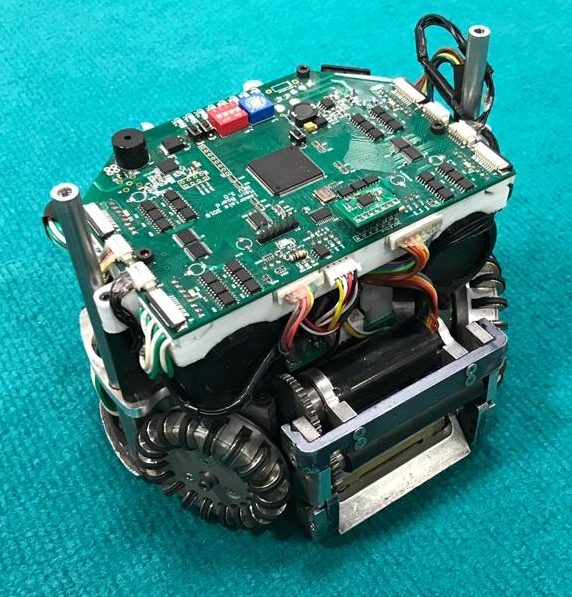
\includegraphics[width=\textwidth]{images/std_robot.jpeg}
         \caption{Standard}
         \label{fig:robot_std}
    \end{subfigure}
    \hfill
    \begin{subfigure}[b]{0.5\textwidth}
        \centering
        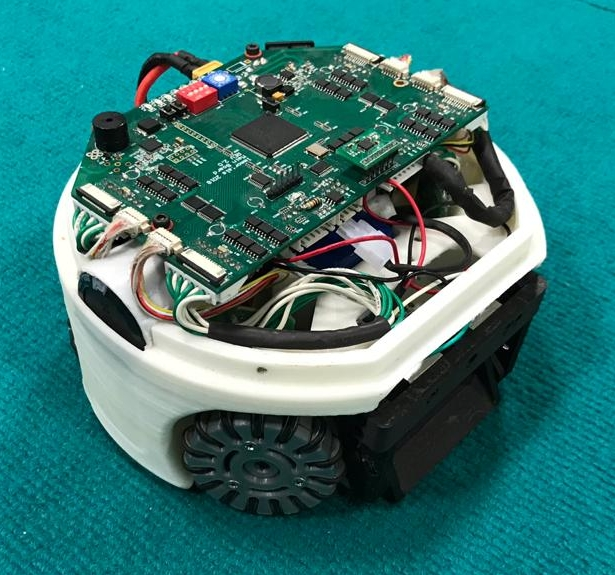
\includegraphics[width=\textwidth]{images/printed_robot.jpeg}
        \caption{3D-printed}
        \label{fig:robot_printed}
    \end{subfigure}
    \caption{Immortals current robots.}
    \label{fig:robots}
\end{figure}

\section {Mechanics}
Due to the optimal design of the previous robots, the mechanical design team decided not to overhaul the entire system, but rather to modify design details to improve the manufacturability and durability of the parts. In addition, recent advances in additive manufacturing techniques, which have resulted in more accurate and reliable 3D-printed parts, are driving our developments toward broader use of these elements and the replacement of several mechanical parts currently manufactured using conventional methods, such as turning and wire EDM, with additively manufactured parts to reduce costs and increase manufacturing and maintenance speeds.

The manufacturing companies are consulted on the technical drawings of the revised design, and most of the manufacturing work for the new series of robots has been outsourced.

\section{Electronics}

Our current electronics were designed in 2010 and have been in use since. In 2018, changes were made to them to modernize the designs and replace the old parts with their new counterparts \cite{ref_ETDP2018}. We tested them during RoboCup 2018, and the results show a solid improvement in reliability while reducing production costs. Currently, all robots use this design.\\
\indent This year, we're planning to redesign all of our electronics from scratch to reflect the latest developments in the league and also in the industry. The main goals are:

\begin{enumerate}
    \item[$\bullet$] reliability
    \item[$\bullet$] expandability
    \item[$\bullet$] being more competitive
\end{enumerate}

\begin{figure}
	\centering
	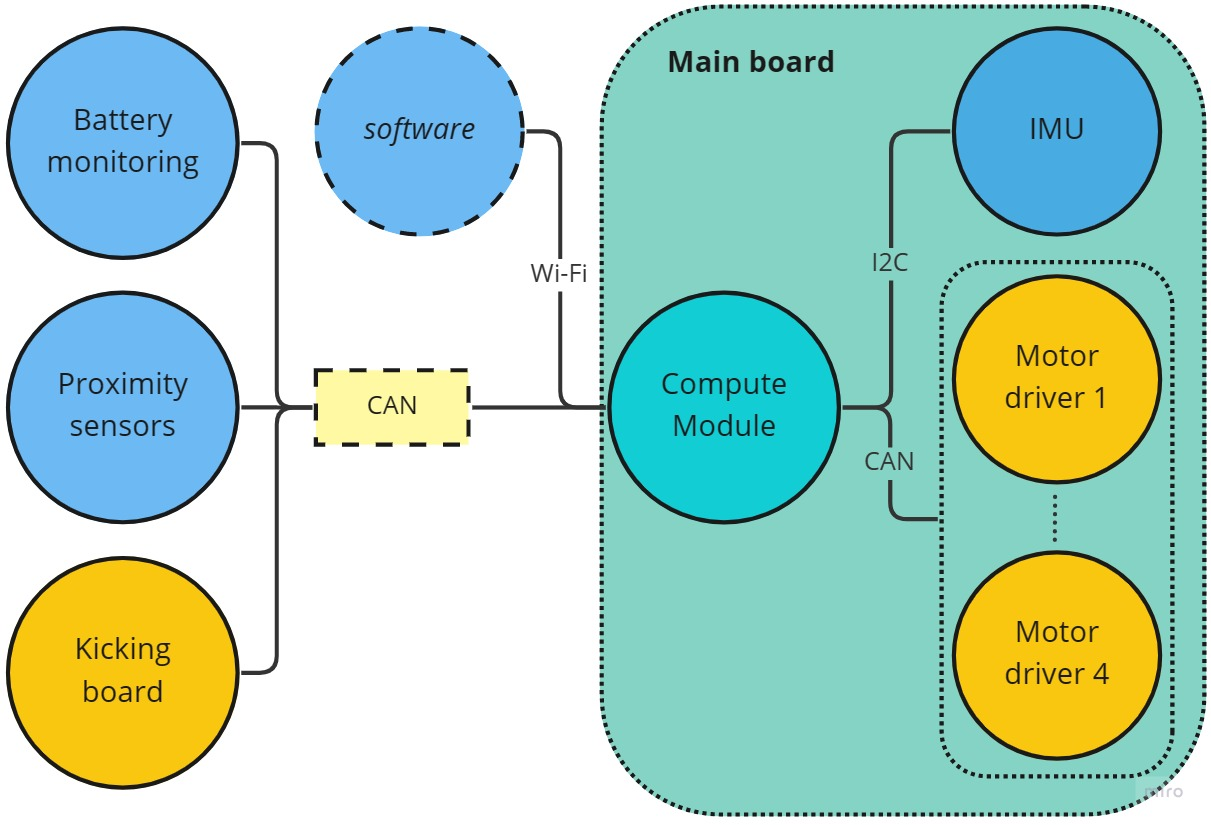
\includegraphics[width=0.8\textwidth]{images/electronics-architecture.jpg}
	\caption{The new electronics architecture}
	\label{fig:electronics-architecture}
\end{figure}

The new architecture can be seen in Fig. \ref{fig:electronics-architecture}. We also switched from the old 4-cell batteries to 6-cell batteries this year. The older batteries were causing the brushless DC (BLDC) motors to run below their rated voltage. But going to a higher voltage was not possible with our previous electronics due to some limitations in the switching power supply we used to generate 5V.

It should be mentioned that at the time of this writing, the design work is still ongoing and we don't have the final boards manufactured. We hope to equip at least half of our robots with the new parts in RoboCup 2023.

\subsection{Main board}
The current main board used by the team was designed in 2010 and has been used in its original form ever since, except for minor changes. It uses a Xilinx Spartan3 FPGA as the main processor. A soft processor, TASKING TSK3000, is used inside the FPGA to handle more sequential logic, while the FPGA itself is used to read encoders, drive BLDC motors, drive the boost converter, etc. We later added an nRF52832 SoC to handle wireless communication, control the I/O switches and LEDs, and read the current sensors \cite{ref_ETDP2018}.

While this design is flexible and comparatively cheap to produce, it has shown its age in recent years. The main drawbacks are:
\begin{enumerate}
    \item[$\bullet$] The TSK3000 runs at about 36 MHz and is far too limited in its current configuration to develop more sophisticated local processing and motion planning. Some effort has been made in the past to move parts of the performance-critical C code to the logic gates, but this would make the implementation more difficult to modify and extend. On the other hand, the debugging workflow was too restrictive, and any changes to the code required a complete rebuild of the FPGA project. All of these factors resulted in the team using pretty much the same framework for several years without being able to make major changes.
    \item[$\bullet$] BLDC motor commutation is a simple 6-step trapezoidal commutation. It is easy to implement, but is inefficient and causes high torque ripples. Implementing a more sophisticated method, such as Field Oriented Control, requires massive changes to the PCB.
    \item[$\bullet$] We use the nRF24L01 chip for wireless communications, with a custom payload layout on top of its Enhanced ShockBurst (ESB) protocol. This gives us a lot of flexibility, but because it is a low-level protocol, we have to add any higher-level functionality we need, such as discovery.
    \item[$\bullet$] The waveform needed to drive the boost converter in the kicking board is generated by the FPGA. This meant that we were free to change it to suit our needs, but in practice, it was considered too fragile.
    \item[$\bullet$] There are no current protections on the board. Any malfunction in the board itself or in any other part of the robot, such as a stuck wheel, will cause damage to the parts. This greatly reduces reliability, increases maintenance costs, and causes damage to the battery.
\end{enumerate}

To resolve these issues the work started on designing a new main board from scratch. The main features are:
\begin{enumerate}
    \item[$\bullet$] Raspberry Pi Compute Module (CM) 4 as the local compute unit on the robot. We intend to move parts of the skill execution, data fusion and prediction, and motion planning to it.
    \item[$\bullet$] Compute Module's 5GHz WiFi as the wireless communication link. This will greatly increase the bandwidth and capabilities of the link and allow us to add robots as regular links to our software stack. This will allow them to receive world state and the AI output necessary to perform local skills.\\
    The latency characteristics of using WiFi instead of a low-level protocol in the lab environment were satisfactory. Using the standard PCB antenna at a distance of 20m from the access point, we were able to achieve a latency of about 2ms with a data loss of about \%3. The latency requirements will be more relaxed after moving more processing to the robot's local processor. However, we are still considering adding a separate nRF chip for latency-sensitive processing if the new approach causes problems.
    \item[$\bullet$] CAN protocol to connect the main board to external boards, including the kicking board, motor drivers, proximity sensors, and battery monitoring. This will give us a more robust and flexible base to build on.
\end{enumerate}

\subsection{Motor driver}
In past competitions, the motor control circuitry was one of the most common points of failure for the robot. Since they were on the same PCB, repairing them would require a complete reflow of the broken parts. In more severe cases, such as when the traces are damaged, especially on the inner layers, this could mean that the board becomes irreparable.\\
This year, we decided to design separate modular motor driver boards that will be placed on the main board for each motor. This will greatly improve our ability to repair robots if one of the drivers fails. It would also make it easier to develop the main board and the motor drivers separately.\\
This new driving board is based on:
\begin{enumerate}
    \item[$\bullet$] A dedicated BLDC motor driver IC, TMC4671. It implements Field Oriented Control (FOC) for BLDC motors and includes various control methods. This offloads the local motor control functionality from the main processor to dedicated hardware, which is more reliable in terms of latency. It has an SPI interface to receive both configuration and commands and to send back sensor data including speed and position.
    \item[$\bullet$] A power MOSFET driver IC, TMC6200. It drives the MOSFETs and senses the motor currents needed for the FOC algorithm. It also includes a fault detection mechanism.
    \item[$\bullet$] A small ARM processor, STM32F042G6Ux, acts as a CAN client link to the main processor. It communicates with both the TMC4671 and the TMC6200 via SPI and also reads the current sensor.
\end{enumerate}

\subsection{Kicking board}
In previous years, we used a boost converter driven by the FPGA from the main board. There were also two discharge pins and one charge pin connected directly to the FPGA's IO pins. These were major problems with this design both in terms of reliability and charge performance.\\

\begin{figure}
	\centering
    \begin{subfigure}[b]{0.45\textwidth}
         \centering
         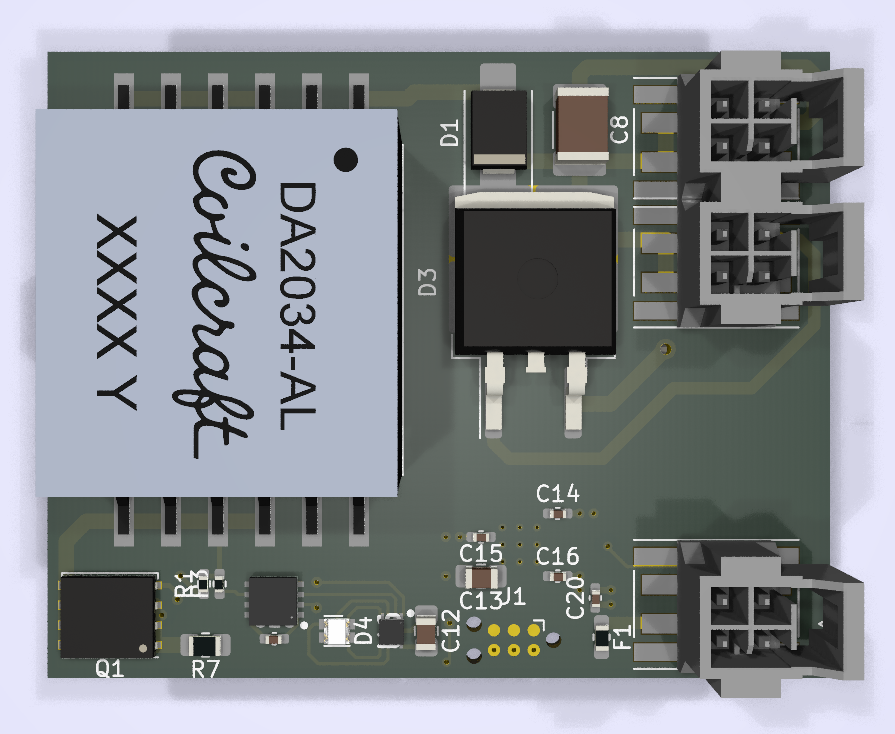
\includegraphics[width=\textwidth]{images/mikona_top.png}
         \caption{top-view}
         \label{fig:mikona_top}
    \end{subfigure}
    \hfill
    \begin{subfigure}[b]{0.45\textwidth}
        \centering
        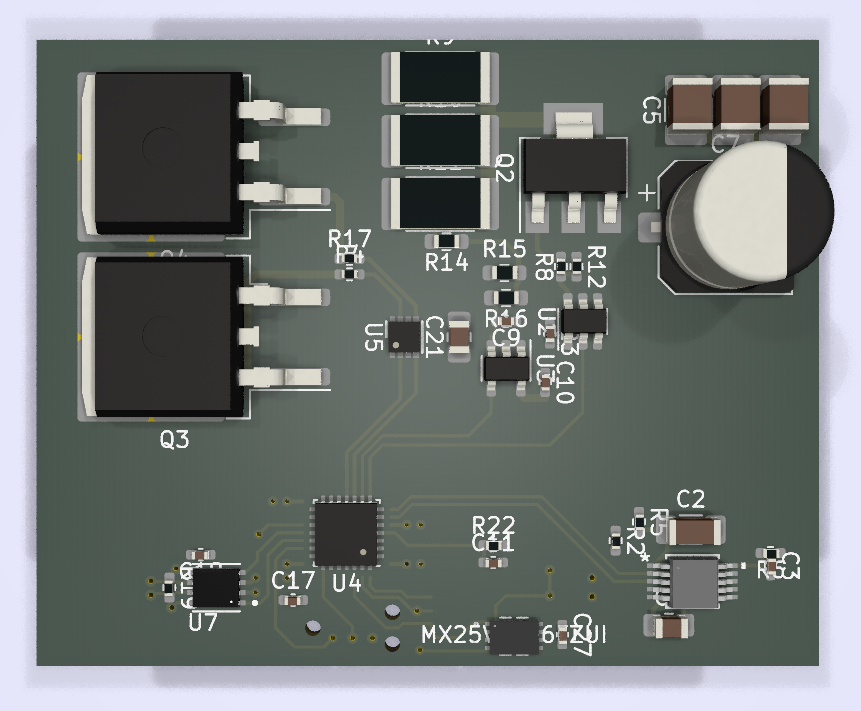
\includegraphics[width=\textwidth]{images/mikona_bottom.png}
        \caption{bottom-view}
        \label{fig:mikona_bottom}
    \end{subfigure}

    \caption{The new kicking board design}
    \label{fig:mikona}
\end{figure}

This year we redesigned the kicking board (Fig. \ref{fig:mikona}) with the following features:
\begin{enumerate}
    \item[$\bullet$] Like other teams in the league \cite{ref_tigers_etdp_2020}, it uses a dedicated LT3570 flyback capacitor charger IC.This simplifies the design while improving performance and reliability. We use the DA2034 transformer and the BSC109N10NS3G MOSFET for this circuit.
    \item[$\bullet$] A STM32F042G6Ux MCU is used on the board to handle the CAN protocol to the main board and to control the charger IC, variable resistors, and discharge IGBTs.
    \item[$\bullet$] A high-power resistor network consisting of three 2.4K 3W resistors is added to the board to discharge the capacitors when needed without using the kicker magnets. The STN3N40K3 MOSFET driven by a ZXGD3009E6 is used to control the discharge.
    \item[$\bullet$] Two IGB50N60T IGBTs driven by a single IX4427MTR are used to discharge the capacitors to the kicking magnets.
    \item[$\bullet$] An MCP4562 variable resistor to set the target voltage of the flyback converter. This allows us to change the voltage by simply changing a configuration variable in the main software and communicating it down to the kicking board.
\end{enumerate}

\section{Software}
Our current software stack was developed in C++ in 2010 and has seen several additions and improvements over the years. This has resulted in a high performance and robust software but at the same time a difficult-to-maintain code base that is too fragile for the new changes.

This year the main focuses are to make our software:

\begin{enumerate}
    \item more robust
    \item easier to read and understand
    \item faster to iterate and extend
    \item more competitive
\end{enumerate}
In the following sections, we will describe the efforts made to reach these goals.

\subsection{Robustness}

\subsubsection{Continuous integration}
\label{section:software_ci}
This year, we created a continuous integration (CI) system based on GitHub workflows. It builds the software, performs style checks, runs automated unit tests, and optionally publishes the result as a release to GitHub. This is an essential part of our development process, as it provides several important benefits that contribute to the quality and reliability of our software.

\indent It helps ensure that the software can be built across environments without problems. This is particularly important as we currently target \textbf{Windows} (\textit{MSVC} and \textit{Clang}), \textbf{Ubuntu} (\textit{GCC} and \textit{Clang}), and \textbf{macOS} (\textit{Clang}) with a collection of library dependencies as will be described in \ref{section:software_3rdparty}. The system uses the same CMake presets that we use locally to ensure that the software is built in a consistent and reproducible way.

\indent It also performs style checks described in \ref{section:software_coding_standard} using clang-format and clang-tidy with the same configurations we use in our local integrated development environments (IDEs). This can help enforce a consistent coding style across the codebase, which can make the code easier to read and maintain.

\indent Another important aspect of the pipeline is the ability to run automated unit tests developed with \textbf{\textit{GoogleTest}} \cite{ref_3rd-party_gtest}. This can help identify problems and regressions in the software early in the development process. At the time of writing, the code coverage of these tests is not adequate and we plan to improve this over time. We also plan to introduce other ways of automated testing other than unit tests in the future, such as testing our tracker with known input and output data, and testing our defensive marking algorithm with situations from the past competitions.

\indent We also have an automatic release submission pipeline when a tag starting with \textbf{\textit{v}}, e.g. \textit{v.1.0.0} is pushed to our repositories. This automatically packages the resulting artifacts, creates a release on GitHub, and publishes the artifact along with the source code and data used to build it. Even this TDP was created using this mechanism.

\subsubsection{Third-party libraries} \label{section:software_3rdparty}
This year we started using several third-party libraries for parts of our software:
\begin{enumerate}
    \item[$\bullet$] \textbf{\textit{BehaviorTree.CPP}} \cite{ref_3rd-party_btcpp} for Behavior Trees
    \item[$\bullet$] \textbf{\textit{Asio}} \cite{ref_3rd-party_asio} for networking
    \item[$\bullet$] \textbf{\textit{Quill}} \cite{ref_3rd-party_quill} for logging
    \item[$\bullet$] \textbf{\textit{toml++}} \cite{ref_3rd-party_tomlplusplus} for configuration files
    \item[$\bullet$] \textbf{\textit{Eigen}} \cite{ref_3rd-party_eigen} for linear algebra
    \item[$\bullet$] \textbf{\textit{homog2d}} \cite{ref_3rd-party_homog2d} for 2D math
\end{enumerate}

\indent Using these libraries over our custom solutions can help improve code quality, both in terms of robustness and ease of use.

\indent These open-source projects have a proven track record and have been extensively reviewed and stabilized over time. This means they are more reliable than custom-built solutions and better suited to handle common tasks with reasonable performance and reliability.

\indent They also often come with a broader set of features that have detailed documentation, making them easier to integrate and use. This allows us to focus on implementing the core logic without worrying about the underlying infrastructure. This results in more readable code that is less prone to bugs.

\indent To make it easier to integrate other libraries, we started using a C++ dependency manager, \textbf{\textit{vcpkg}} \cite{ref_3rd-party_vcpkg}. This simplifies the installation and maintenance of third-party libraries, ensures compatibility between them, and improves reproducibility on different local machines and in the CI pipeline.

\subsubsection{Improved debugging}
One of the main weaknesses of our software in the previous competition was the lack of understanding of why the software and robots were behaving the way they were and what might be causing the problems we were seeing. We knew that by providing more detailed and informative logs, we could gain a better understanding, which could lead to faster and more effective debugging and troubleshooting.

This year, we improved our logging system with an extensible system that can output to multiple outputs, including the standard output, file, and over the network. This allows us to record the logs and later analyze any part of the runtime to better understand the behavior of the system and narrow down the problem to a specific point in time.

We have also expanded the use of our visualization GUI. Having a graphical representation of the internals of different algorithms, as well as real-time sensory data from the robots, help us better understand how different parts of the software work and make more informed decisions about how to improve the robots' performance and troubleshoot problems. The GUI also provides a more intuitive and user-friendly way to interact with the software and make configuration changes. Fig. \ref{fig_visualizer} shows an example of visualizing the internals of our path planning.

\begin{figure}
    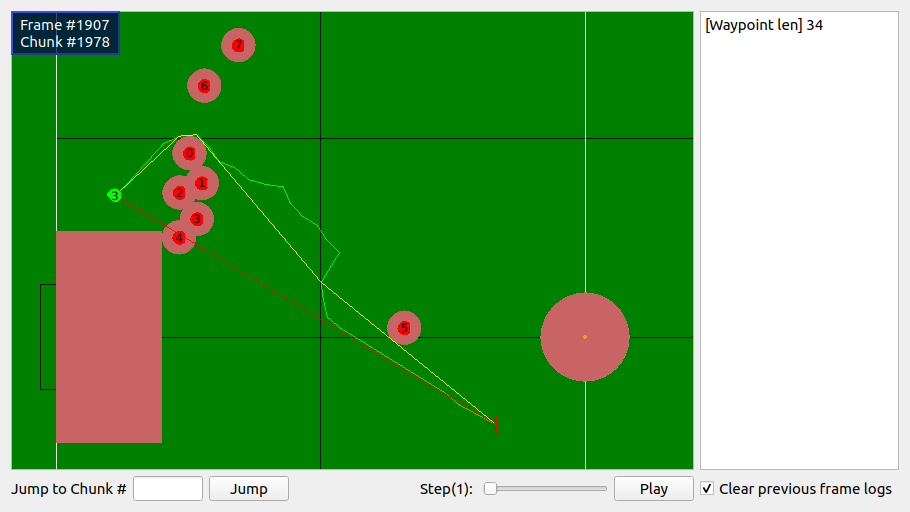
\includegraphics[width=\textwidth]{images/visual1.png}
    \caption{A demonstration of the ERRT path plan in the visualization GUI.}
    \label{fig_visualizer}
\end{figure}

The GUI is implemented in Python and receives the visualization data over the network. This means that it can be run on any computer in the same network and receive the data from any node in the system, including the tracker, the soccer ball, and even the robots' embedded firmware.


\subsection{Readability}

\subsubsection{Architecture}
Our current software is a single monolithic application that handles world state estimation, AI, and robot motion planning. This has the advantage of allowing us to easily change the flow of data between different parts. But it forces us to implement everything in C++ to produce a single application that runs on a single machine. Another side effect of such a monolithic design was that it encouraged more coupling between the soccer and vision parts of the software, making it harder to make changes to either.

\begin{figure}
	\centering
	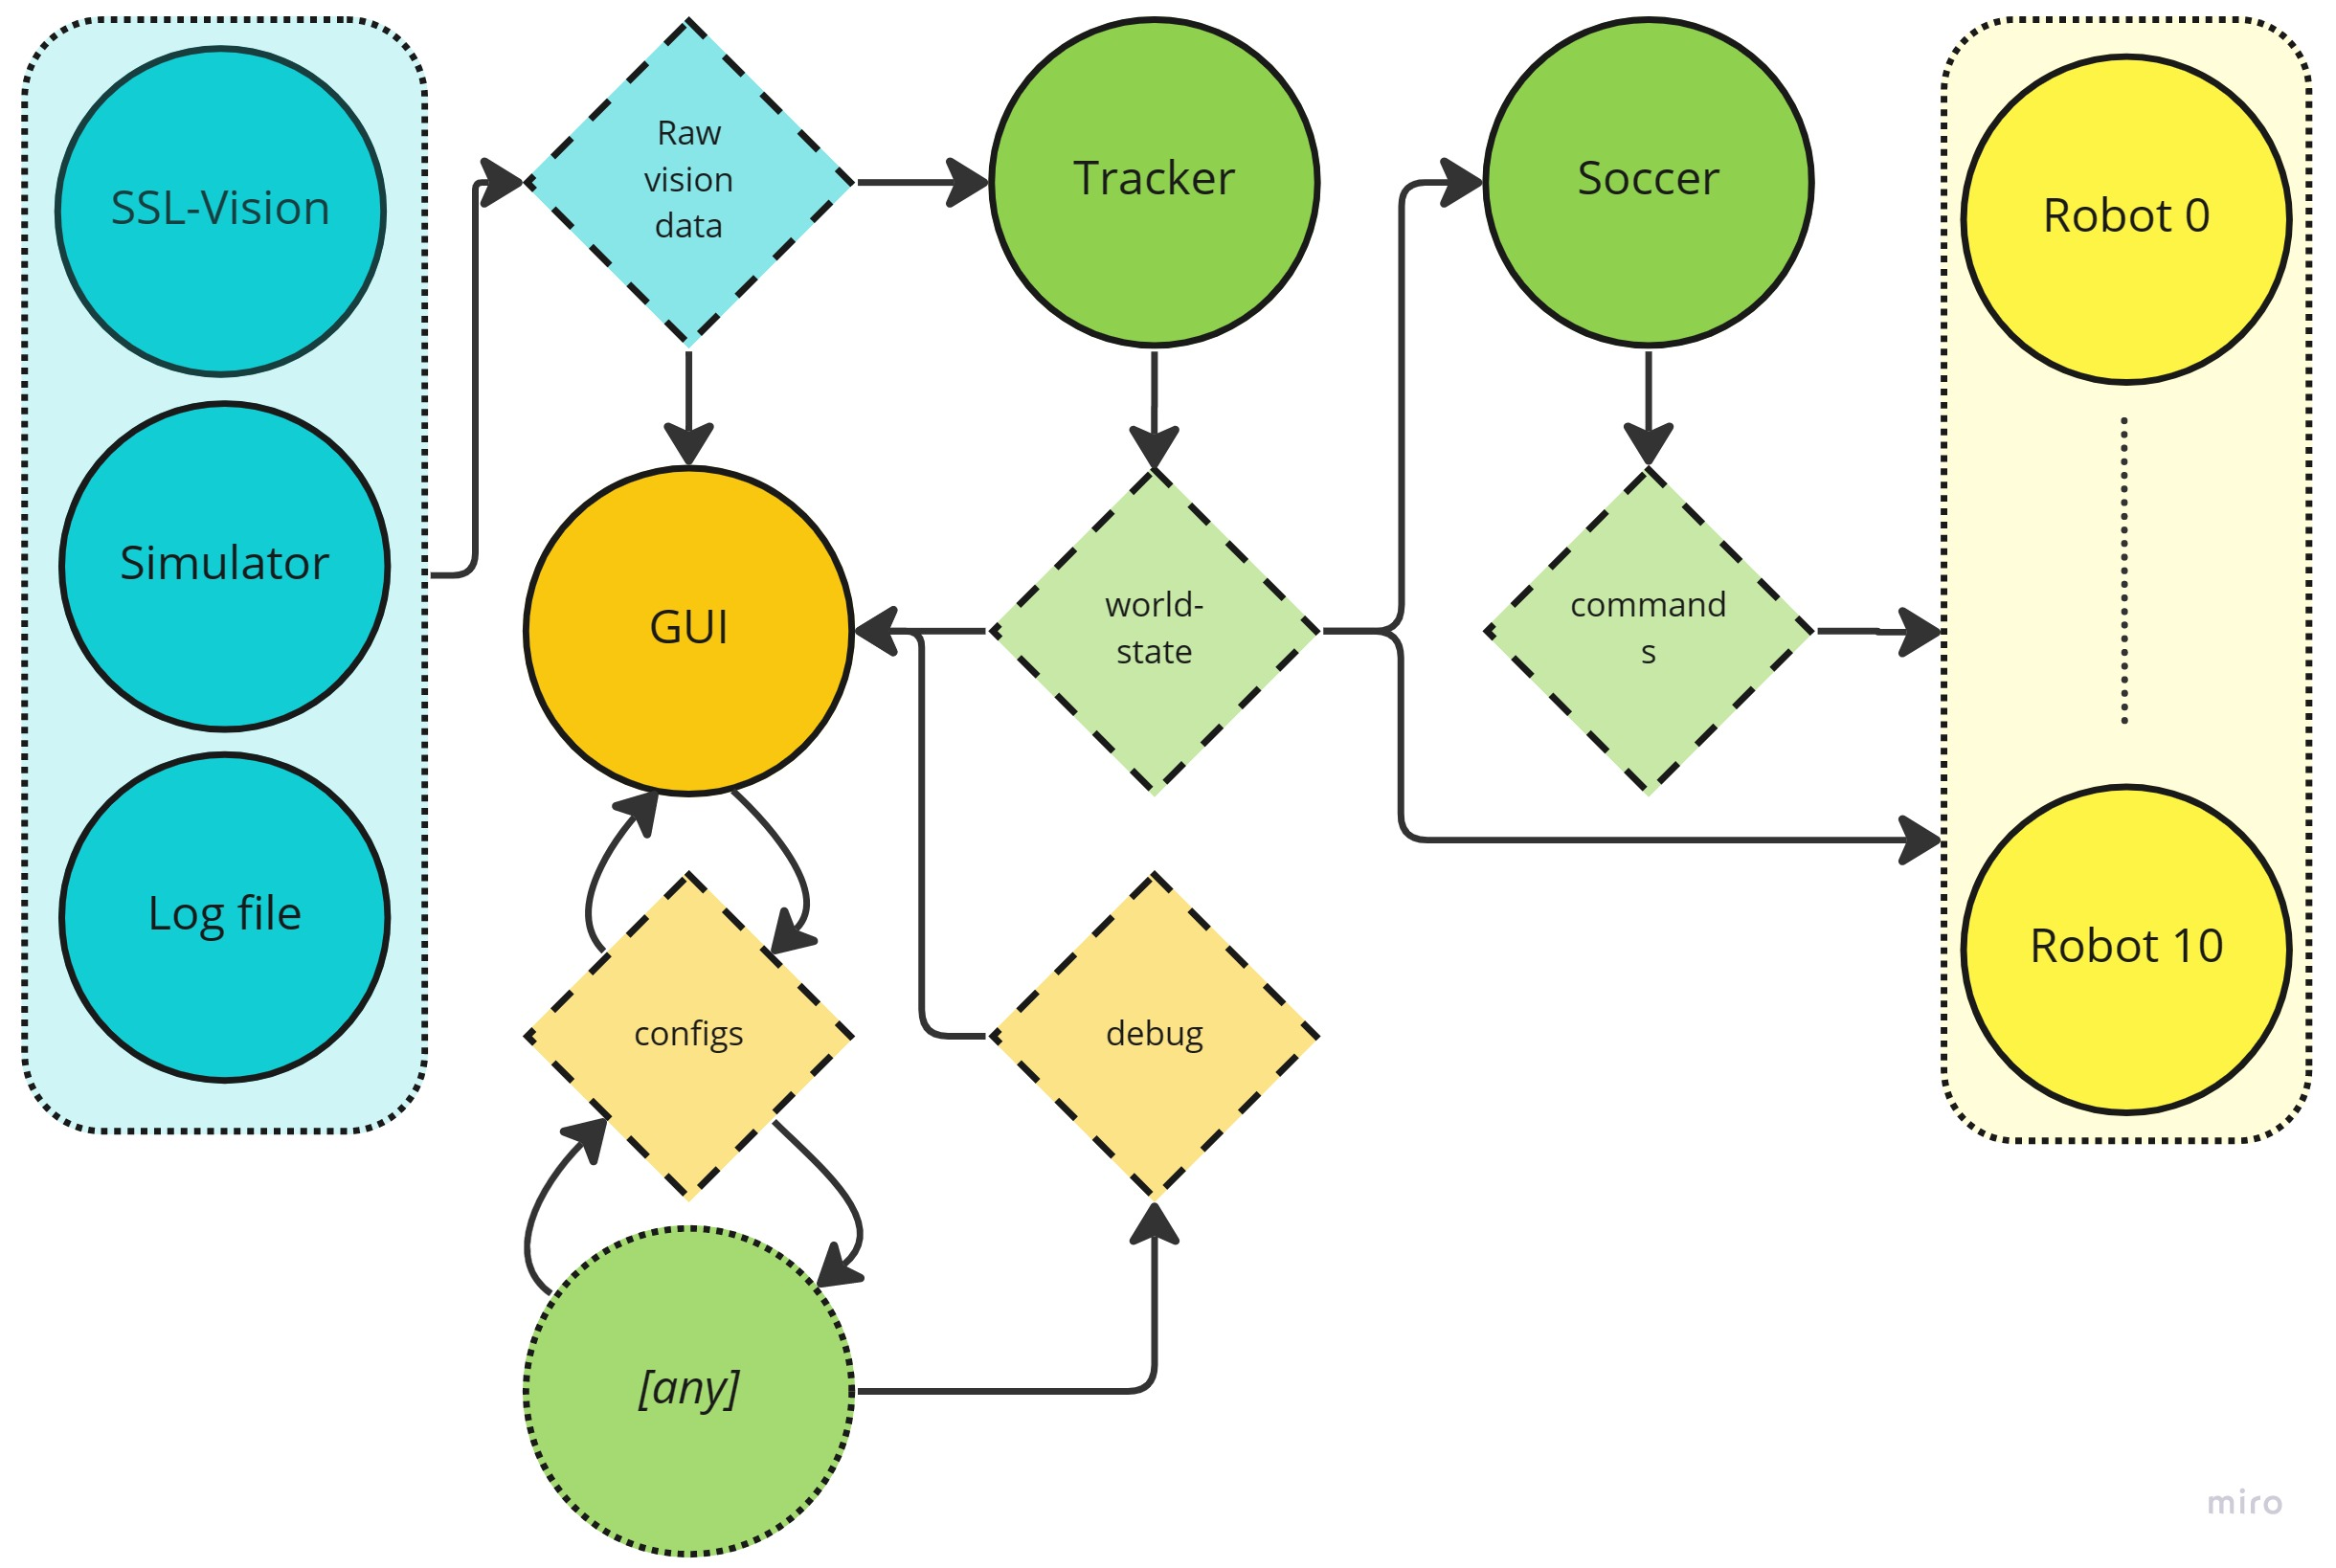
\includegraphics[width=0.9\textwidth]{images/software-architecture.jpg}
	\caption{The new software architecture}
	\label{fig:software-architecture}
\end{figure}

The goal this year is to refactor the code base into separate parts that are connected via the network as shown in Fig. \ref{fig:software-architecture}. This will allow us to move the lower-level motion planning and skill execution to the robot's local processor and develop the graphical user interface (GUI) using other technologies.

At the time of writing, these efforts are still ongoing, but we are confident that we will be able to transition to the new stack in time for RoboCup 2023.

\subsubsection{Coding standards}
\label{section:software_coding_standard}
One of the most important observations in the past has been the complexity of the C++ language and the large number of problems that can arise when it is used incorrectly. This is especially important to us because the code is typically developed by students who do not have extensive experience with the language.

To address this issue, we have chosen a coding standard \cite{ref_cppbestpractices} and agreed on a set of style and naming conventions to be used throughout the code base. These will improve readability and maintainability, and promote consistency. These style checks are implemented as \textbf{\textit{clang-tidy}} and \textbf{\textit{clang-format}} configurations which can be used both locally within the IDEs, and as an automated gate in our CI pipeline as described in \ref{section:software_ci} when creating a pull-request to the main branch.

As a first step in implementing the coding standard, we have begun to move the code base to a more modern C++ revision (C++20 at the time of this writing). It includes as an example moving away from the use of raw pointers in favor of smart pointers. This can help simplify memory management, improve code clarity and maintainability, and reduce the risk of errors related to object ownership and lifetime.

We are also in the process of making the code base warning-free and treating the new warnings as bugs. These warnings are issued by the compiler when it detects potential problems in the code that could lead to bugs or undefined behavior based on the C++ Core Guidelines \cite{ref_cppcoreguidelines} or other references. Treating them as errors force developers to address them and fix potential problems early in the development process, which can help prevent the accumulation of technical debt and reduce the risk of introducing bugs later.

\subsection{Extensibility}

\subsubsection{Issues with Finite-State Machines}
Our current AI is based on finite-state machines (FSMs) \cite{ref_ETDP2020}. While this structure made it easier to decompose robot behavior into distinct states and implement each event as a transition between two states, it made it difficult to reuse states and increased the number of transitions exponentially. It also became very difficult to debug or extend the FSM to handle new behaviors and implement fallback tactics.

When implementing each state of an FSM, the developer must consider the other states and how they will transition to the current state and how it will transition to the next state. For a state machine with only a few states, this is easier to handle. However, considering the number of robots and the different tactics that the opponent can use, the developer is required to implement a large number of states to handle every possible situation in the FSM. This can be a significant challenge for the developer to implement all the states and their relationships.

\subsubsection{Behavior trees}
To overcome these problems, we switched to Behavior Trees (BT) this year. BTs are hierarchical structures composed of nodes representing actions, conditions, or other behaviors, and their connections define the order in which those behaviors should be executed. BT can be used to develop AI for soccer-playing robots by providing a framework for creating complex decision-making algorithms that can handle multiple goals and constraints.

\begin{table}
    \centering
    \footnotesize
    \caption{Low-level behaviors.}
    \label{tab:low-level-behaviors}
    \begin{tabular}{|p{0.5\textwidth}|p{0.45\textwidth}|}
        \hline
        \bf{Behavior} & \bf{Description} \\
        \hline
        {\itshape Navigate(destination, orientation, profile)} & Navigate the robot to \textit{destination} with the provided velocity \textit{profile} while avoiding obstacles.\\
        {\itshape Chip(power)} & Request a chip kick with the passed \textit{power} to be executed when the ball is detected.\\
        {\itshape Direct(power)} & Request a direct kick with the passed \textit{power} to be executed when the ball is detected.\\
        \hline
        {\itshape Obstacles(situation)} & Returns obstacles for the robot for a given \textit{situation} in the game.\\
        {\itshape Face(point)} & Returns an orientation so that the robot faces the passed \textit{point}.\\
        {\itshape Mark(opponent)} & Returns the defensive marking position for the given \textit{opponent} that is either between our goal and the \textit{opponent}, or the ball and the \textit{opponent}.\\
        {\itshape FetchBall(point)} & Returns the position on line which the ball is moving on and most close to the \textit{point}, and an orientation to fetch the ball.\\
        {\itshape OneTouch(point, target)} & Returns the position on line which the ball is moving on and most close to the \textit{point}, and an orientation to kick the ball towards the \textit{target}.\\
        \hline
    \end{tabular}
\end{table}

Table \ref{tab:low-level-behaviors} shows the low-level behaviors that can be used as building blocks to create more complex behaviors. They are self-contained and easy to understand, so they can be developed and tested once, which is much less time-consuming than maintaining complex and interconnected systems developed together.

Fig. \ref{fig:bt-move} shows an example BT that is built upon the lower-level behaviors described earlier in table \ref{tab:low-level-behaviors}. Note that this tree is stored as an \textit{XML} file that the software can load and reload at runtime, without a need to recompile. This greatly improves the iteration times.

\begin{figure}
	\centering
	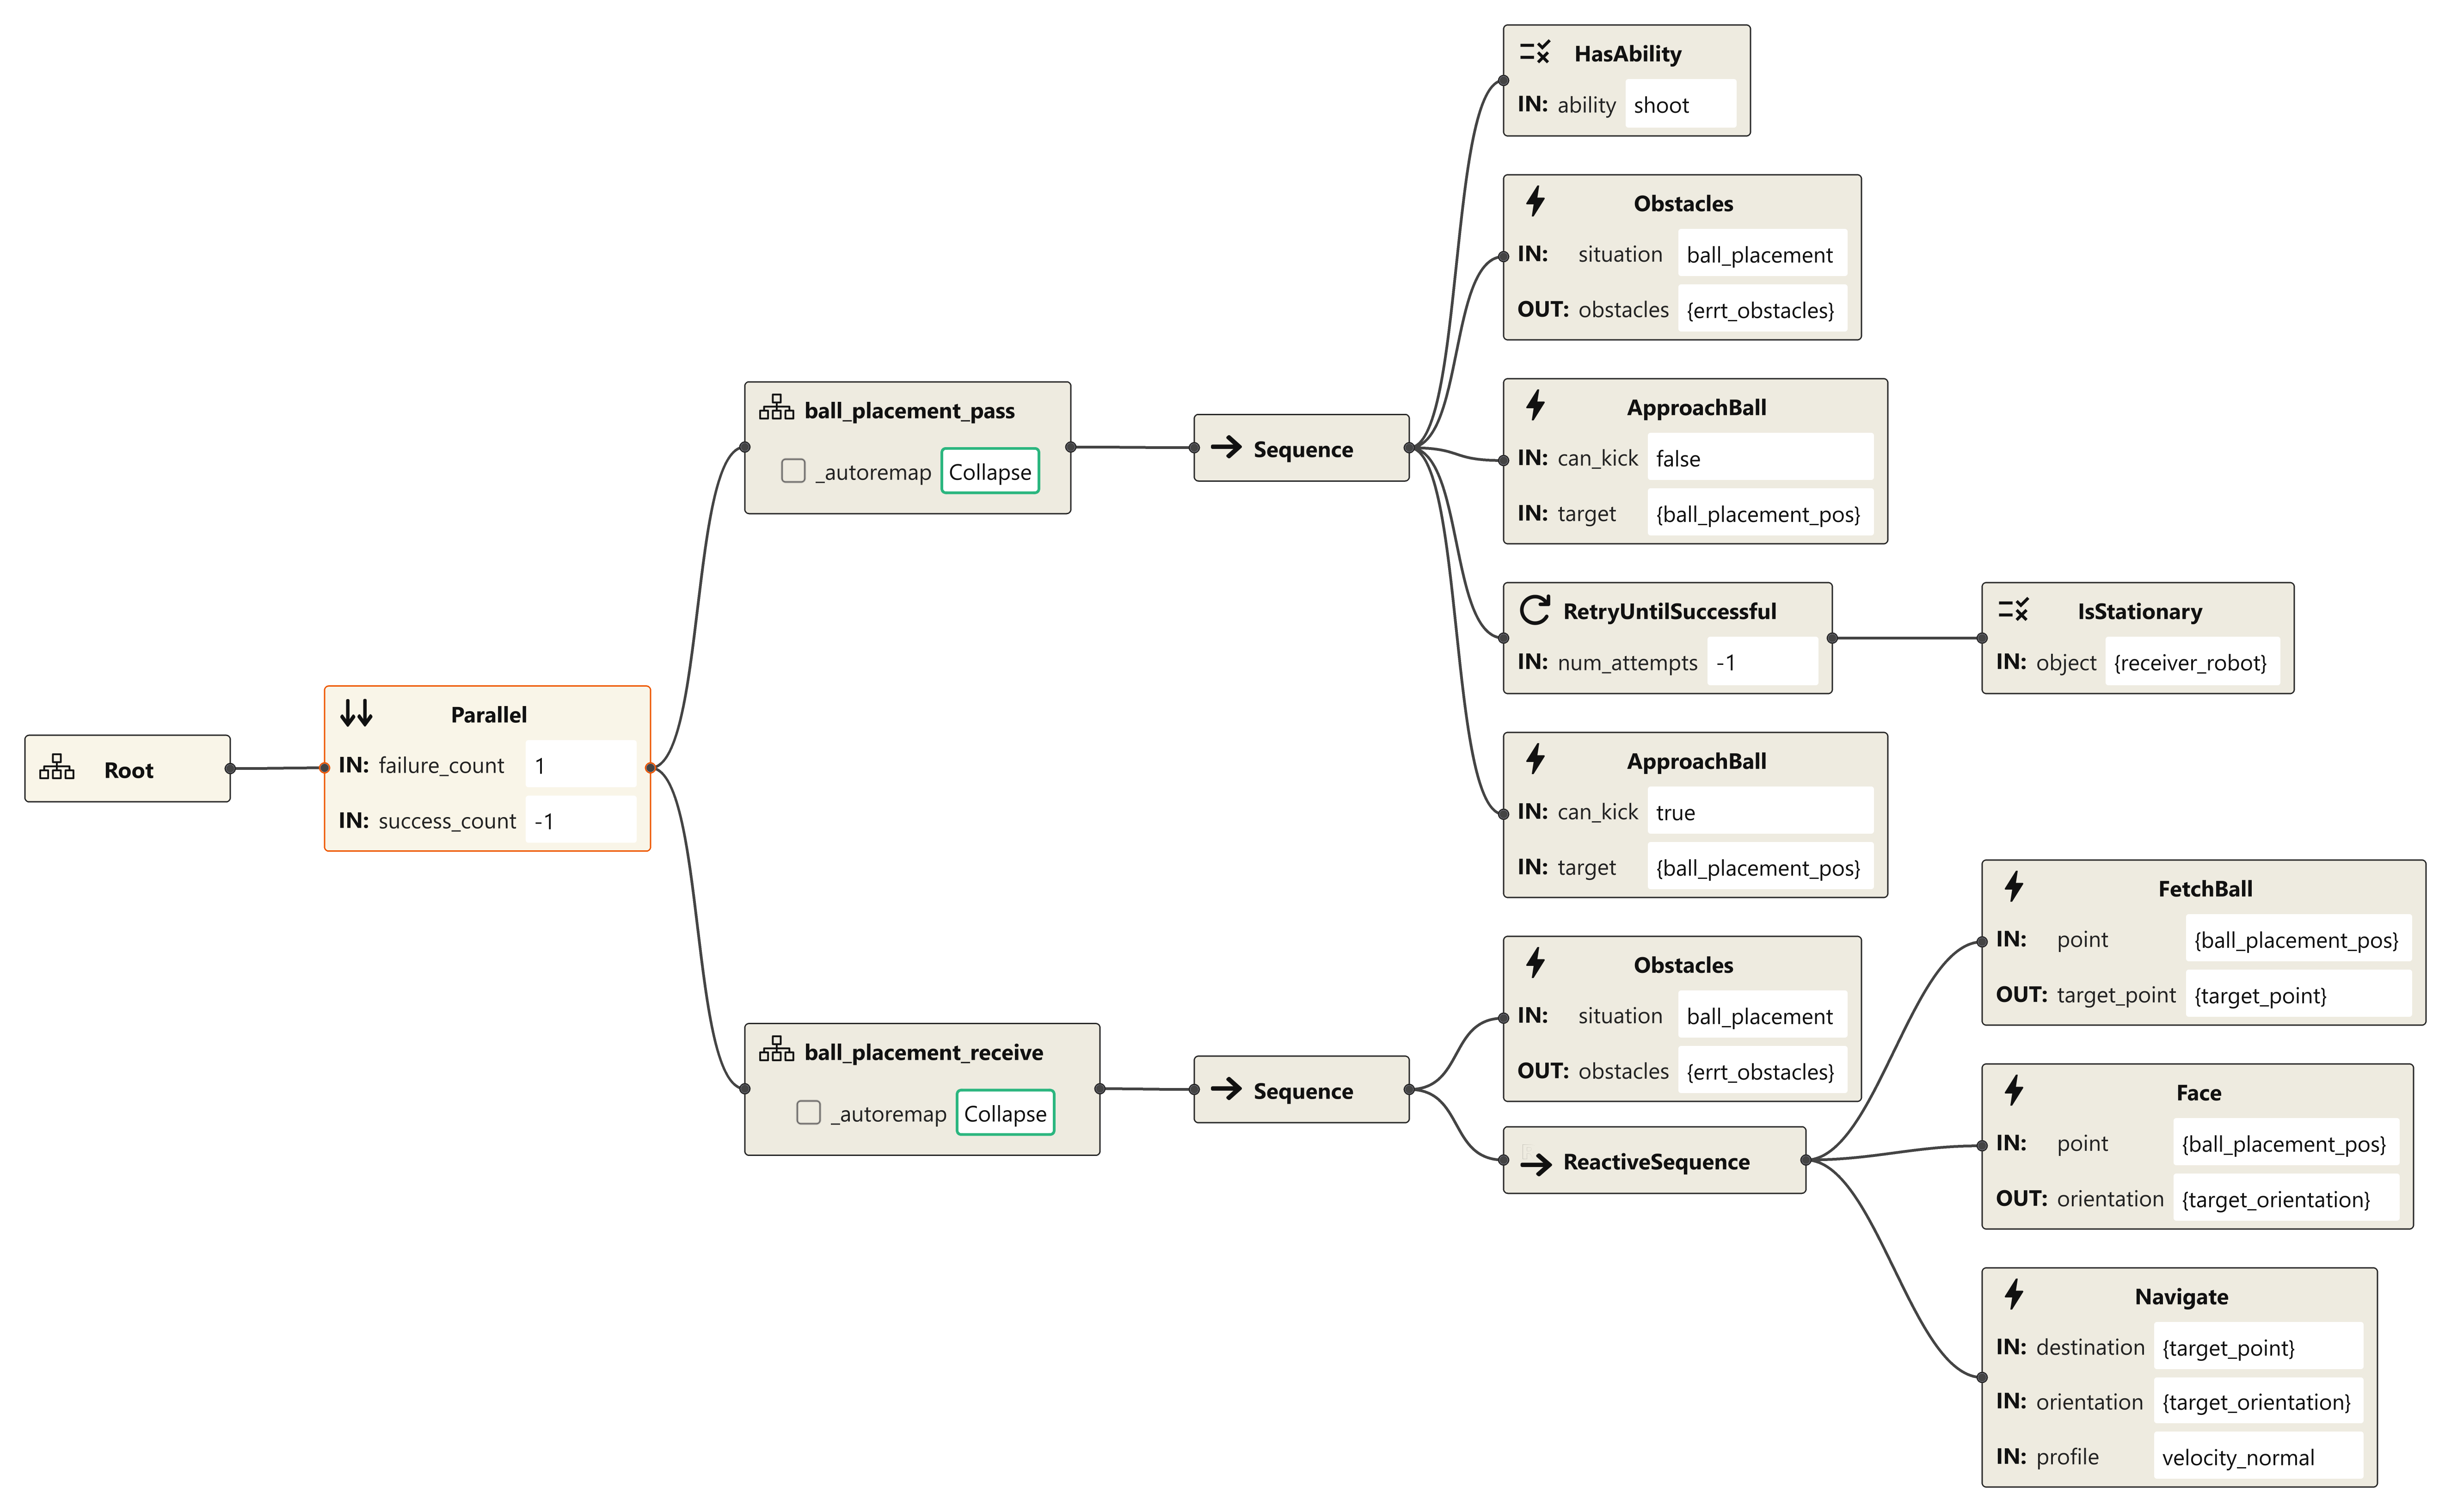
\includegraphics[width=0.95\textwidth]{images/ball_placement_bt.png}
	\caption{A sample Behavior Tree for ball placement.}
	\label{fig:bt-move}
\end{figure}

By using BTs in the development of our AI, we can create flexible, modular, and easy-to-maintain decision-making algorithms that can handle the complexity and variability of the games. The hierarchical structure of the BT also allows for a high degree of customization and adaptability, making it easier for us to adjust our strategy based on the specific conditions of each game.

\subsubsection{Config system}
Previously, all parameters were hard-coded into the C++ code. This made it time-consuming to change anything, resulting in unacceptably long iteration times. Using a config file instead makes it easier to maintain and update the values, as they can be changed in a central location instead of having to search for each instance of the hard-coded value. It also makes the code more flexible and reusable, since you can easily switch between different configurations without having to change the code itself. This also makes it easier to test different scenarios without restarting the system.

This year we started using \textbf{\textit{toml}} \cite{ref_toml} as our configuration format, along with a \textbf{\textit{json schema}} \cite{ref_json-schema} that we generate based on our C++ config structure to validate the toml file in both text editors and as a CI step. This schema is also used by our GUI to create a persistent config editor with the correct types, names, and defaults, even in the absence of a config file. The system uses a layered architecture; multiple toml configs, both from disk files and from the network, are fed into the system, each with a priority field. The configuration system then returns a single compiled configuration that all nodes in the system can use (Fig. \ref{fig:software-architecture}). The system can also prompt the nodes in the system to persist the received config.

\subsubsection{Improving build time}
One of the common pitfalls of any C++ code base is the time it takes to build the project. This problem became more apparent as our software grew in size and dependencies. Before doing any optimizations, it took about 15 minutes to do a complete rebuild on a modern desktop CPU with 6 physical and 12 logical processors.

As a first step, we enabled multi-threaded compilation with \textbf{\textit{/MP}} flag on MSVC and using \textbf{\textit{Ninja}} \cite{ref_ninja} instead of make. This greatly reduced the build time to about 3 minutes. But it was still unacceptable for the iteration times we were looking for.

\begin{figure}
	\centering
	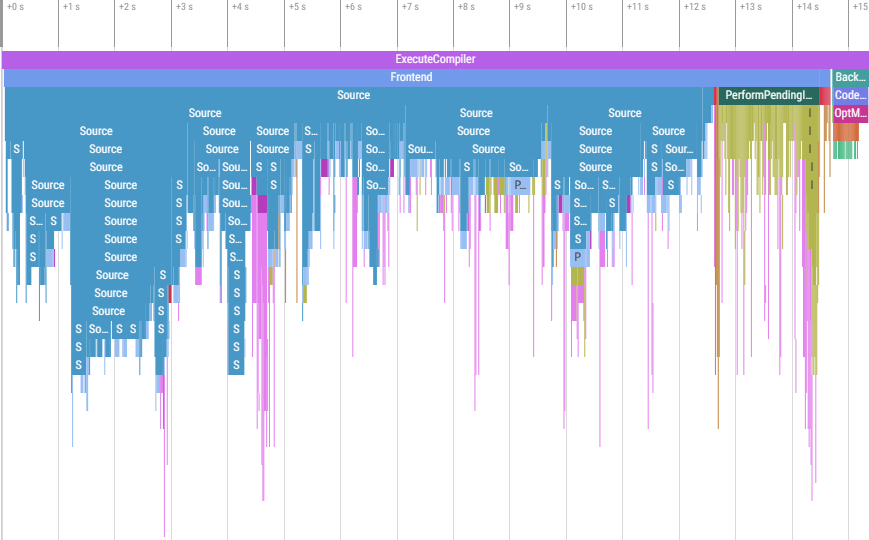
\includegraphics[width=\textwidth]{images/time-trace.png}
	\caption{The output of the \textit{-ftime-trace} for one of the source files.}
	\label{fig:time-trace}
\end{figure}

We then used the \textit{-ftime-trace} flag with Clang to see where the time is spent during the build. As shown in Fig. \ref{fig:time-trace}, most of the time is spent in the frontend, in this example about \%96 of it. Upon closer inspection, it is clear that this is caused by excessive use of include files, which the compiler frontend has to process multiple times.

To solve this problem, we started using \textit{unity build}, so that the headers are processed once for a set of source files. This resulted in a massive reduction in build times. A full rebuild took about 20 seconds on the same machine. But touching a single source file still triggered the compilation of a set of files, which is inefficient.

The last step to improve build time was to use \textit{pre-compiled header} (PCH). All header files from the 3rd party libraries, and the common code used by both vision and soccer modules except the generated protobuf header files are pre-compiled. This is then used by the compiler when compiling the vision and soccer modules. This way, the time to do a full rebuild is almost the same as the unity build. But the time to build the modules when only a few source files are changed became about 2 seconds, which shows a reduction of about \%80 compared to the unity build.

We currently use PCH locally, and unity builds together with PCH for our CI pipeline.

\subsection{Competitiveness}
As mentioned earlier, the main focus this year has been to improve the foundation of our code base to make it easier to build more competitive software on top of it. We expect to see more soccer-related development in the coming years. The following sections describe the work we expect to be done in time for RoboCup 2023.

\subsubsection{Local processing on robots}
Currently, we run all the behaviors in the main software on a computer, and then send the target commands in the form of global target velocity, orientation, and kick commands to the robots. The robot's local processor then performs sensor fusion on the orientation processed by the vision and the local Inertial measurement unit (IMU). This greatly improves the quality of the predicted orientation.

To extend this idea, we plan to do more sensor fusion on the robot. We will use the output of the four rotary encoders connected to the wheels, the output of the IMU, the proximity sensor array around the robot, and the filtered world state received from the tracker.

In addition, we want to move most of the low-level behaviors shown in table \ref{tab:low-level-behaviors} to the robot's local processor. Combined with local sensor fusion, this results in improved navigation efficiency and safety, even in the presence of excessive vision noise and wireless link latency variations.

\newpage
\begin{thebibliography}{8}
\bibitem{ref_ETDP2020}
Immortals 2020 Extended Team Description Paper, \url{https://ssl.robocup.org/wp-content/uploads/2020/03/2020\_ETDP\_Immortals.pdf}.

\bibitem{ref_ETDP2019}
Immortals 2019 Team Description Paper, \url{https://ssl.robocup.org/wp-content/uploads/2019/03/2019\_ETDP\_Immortals.pdf}.

\bibitem{ref_ETDP2018}
O. Najafi Koopai, M.A. Ghasemieh, M. Khanloghi. Immortals 2018 Team Description Paper.

\bibitem{ref_tigers_etdp_2020}
Ryll, Andre and Jut, Sabolc. TIGERS Extended Team Description for RoboCup 2020


\bibitem{ref_github}
Immortals Open Source Project. \url{https://github.com/Immortals-Robotics}.

\bibitem{ref_cppbestpractices}
Turner, Jason. "C++ Best Practices"

\bibitem{ref_cppcoreguidelines}
Stroustrup, Bjarne and Sutter, Herb. "C++ Core Guidelines"

\bibitem{ref_toml}
TOML, A config file format for humans. \url{https://toml.io/}.

\bibitem{ref_json-schema}
JSON Schema, a declarative language that allows you to annotate and validate JSON documents. \url{https://json-schema.org/}.

\bibitem{ref_ninja}
Ninja, a small build system with a focus on speed. \url{https://ninja-build.org/}.

% 3rd-party libraries
\bibitem{ref_3rd-party_gtest}
GoogleTest, Google Testing and Mocking Framework \url{https://github.com/google/googletest}

\bibitem{ref_3rd-party_vcpkg}
vcpkg, cross-platform C/C++ dependency manager from Microsoft \url{https://vcpkg.io/}

\bibitem{ref_3rd-party_btcpp}
BehaviorTree.CPP, a C++ library to build Behavior Trees. \url{https://www.behaviortree.dev/}

\bibitem{ref_3rd-party_asio}
Asio, cross-platform C++ library for network and low-level I/O programming \url{https://think-async.com/Asio/}

\bibitem{ref_3rd-party_quill}
Quill, asynchronous Low Latency C++ Logging Library \url{https://github.com/odygrd/quill}

\bibitem{ref_3rd-party_tomlplusplus}
toml++, header-only TOML config file parser and serializer for C++17. \url{https://github.com/marzer/tomlplusplus}

\bibitem{ref_3rd-party_eigen}
Eigen, C++ template library for linear algebra \url{https://eigen.tuxfamily.org/}

\bibitem{ref_3rd-party_homog2d}
homog2d, C++ 2D geometry library \url{https://github.com/skramm/homog2d}

\end{thebibliography}
\end{document}
